\documentclass[runningheads]{llncs}
\usepackage[T1]{fontenc}
\usepackage{graphicx}
\usepackage{listings}
\lstset{breaklines=true, language=C}
\raggedbottom
\begin{document}
%
\title{MitTorrent}
\author{Mitreanu Alexandru}
\institute{Faculty of Computer Science, Romania, Iasi}

\maketitle

\section{Introduction} \label{intro}
This section presents the purpose of this project. MitTorrent is my personal implementation of the Part2Part project. It is a peer-to-peer file transfer application. The purpose of this application is to provide users with a method of transferring files between remote clients, while trying to make efficient use of the client's resources.

\section{Applied Technologies} \label{applied_technologies}
The application uses the TCP protocol for all connections, because it is important to have reliability for all types of communication (be it simple requests or file transfer requests).

The application implements the Chord protocol \cite{ref_url10}. It uses it in order to distribute the file information across nodes in the network as will be described in a further section in more detail.

The application doesn't use any other external technologies besides the POSIX and C standard libraries.

However, a logger, an error system, data structures such as linked lists and vectors, a command parser and other small libraries are implemented to facilitate easier development along the way.

\section{Application Structure} \label{app_structure}
\subsection{Chord protocol} \label{chord_protocol}
The Chord protocol assigns identifiers to keys and nodes. The identifiers are placed in an identifier circle modulo $2^m$, where $m$ is the number of different ids that can exist. The successor of a key is the first node that has an identifier equal or greater than the one of the key. If we look on the identifier circle, the successor of a key is the first node that has an identifier equal or greater than the key going clockwise. This is how the protocol maintains a roughly equal amount of load on each node. In my implementation the nodes are trackers and the keys are ids of the torrent files.

\subsection{Operations} \label{operations}
\subsubsection{Upload.}
When a tracker wants to upload a file to the network, it must first create a torrent file for it, which should contain relevant information about the file: id, name, size and the list of peers that own the file (initially only the tracker owns the file). After the torrent file is created, the id, name and size of the file are sent to the server to allow trackers and non-trackers to search for files by id, name and size. After that, the tracker uploads the torrent file to the network, by using the Chord protocol. What it does is finding the successor node of the torrent file key. That node is responsible for holding the torrent file and giving it to other peers if they want to download the file. Non-trackers are not allowed to upload files.
\subsubsection{Search.}
When a non-tracker or tracker wants to search a file on the network, it must ask the server to look through it's list of uploads. The server will give a list of responses to the client, each response containing the id, name and size of the torrent file, these ids will be used for downloading.
\subsubsection{Download.}
When a non-tracker wants to download a file, it must ask the server to find the successor of a given torrent file id by asking one of the nodes that are on the network (because the server keeps track of all trackers) and tell the client the address of that successor. For a tracker it can ask directly on the network to find the successor. After the address of the successor is retrieved, both a non-tracker and tracker will ask the tracker that owns the torrent file to give it to them. After that, the download can start.

\subsection{Download protocol} \label{download_protocol}
The download protocol is defined as follows. Each file is split into blocks. A client that wants to download a file will use the downloader module to download that file. The downloader module takes a torrent file, asks each peer from the peers list what blocks of that file it owns. Then it uses an algorithm to decide which peers to ask for which blocks and starts retrieving blocks from other peers. After the algorithm is over there are two states possible: either the download is complete or not. In the second case, the user may retry the download at any point following the same procedure as above. There is also the possibility of stopping downloads at any moment. Each download is done on a separate thread, there is a cap on the max number of downloads that can be done in parallel.

\subsection{Server Structure} \label{server_structure}
The server is composed of two components: the main module and the API module.
\subsubsection{The main module}
uses the command parser module to allow the server admin to run commands on the server.
\subsubsection{The API module}
is effectively the server to which clients will connect. The server handles requests concurrently. The server keeps track of all trackers connected to it using a list and it also keeps information about all uploads that occurred on the Chord network in order to allow searching by criteria such as id, name and size (with the possibility of adding more fields).

\subsection{Client Structure} \label{client_structure}
The server has three components: the main module, the downloader module and tracker module
\subsubsection{The main module}
takes care of user input by using the command parser module in order to allow clients to run commands.
\subsubsection{The downloader module}
handles downloading of files as described in \ref{download_protocol}.
\subsubsection{The tracker module}
makes the difference between a tracker and a non-tracker. A non-tracker does not implement this module. This module allows a client to become part of the Chord network.

\subsection{Application Diagram} \label{app_diagram}
\begin{figure}
\includegraphics[width=\textwidth]{diagram.drawio-2.pdf}
\caption{Application diagram} \label{app_diagram_fig}
\end{figure}

\pagebreak

\section{Implementation Aspects} \label{implementation}
\subsection{Command parser}
Found in \verb|cmd_parse.h|.

The project has a command parsing library which breaks a command into tokens in order to allow the clients and server admins to run commands easily. A command looks like this: \verb|cmd_name [-flag [value]]...|

\subsection{Key type} \label{key2_t}
Found in \verb|key.h|.

The ids for used in the Chord protocol are computed as a SHA256 hash \cite{ref_url1} over the \verb|sockaddr_in| field of a node or over the contents of a file that is to be uploaded on the network. The following methods are used for this:
\begin{lstlisting}
void key_from_addr(key2_t *key, struct sockaddr_in *addr);
int32_t key_from_file(key2_t *key, int32_t fd, uint64_t *size);
\end{lstlisting}

\subsection{Chord protocol}
Found in \verb|dht.h|.

First, we must distinguish between two types of nodes: local and remote. The \verb|node_remote_t| type is defined as follows:
\begin{lstlisting}
typedef struct {
    key2_t id;                      // key of peer
    struct sockaddr_in addr;        // connect info of node
} node_remote_t;
\end{lstlisting}
All we need to know about a node is it's id in the identifier circle and it's address for connection through sockets.

We will also need to define the notion of finger. Each node has $log_2(m)$ fingers which are used for faster look-ups on the identifier circle. The $i^{th}$ finger starts at position $node.id + 2^{i-1}$ (mod $2^m$). Each finger stores the successor of this starting position. This way we have some routing information for lookup requests. The \verb|finger_t| type is defined as follows:
\begin{lstlisting}
typedef struct {
    int32_t initialized;            // specifies if the entry has been inited or not
    key2_t start;                   // (node.id + 2^(i-1)) mod 2^m
    node_remote_t node;             // can be either local or remote
} finger_t;
\end{lstlisting}
The \verb|node| field is filled with the successor of \verb|start|. \verb|initialized| is a flag used internally to avoid fingers that are not initialized to speed up look-ups.

Now we can define what a local node is. A tracker, in order to make part of the Chord network, must hold some state regarding the network, as such we have the \verb|node_local_t| type:
\begin{lstlisting}
typedef struct {
    key2_t id;                      // key of peer
    struct sockaddr_in addr;
    finger_t finger[KEY_BITS];
    int32_t prev_initialized;       // can be set to nil
    node_remote_t prev;
} node_local_t;    
\end{lstlisting}
The first two fields match the definition of \verb|node_remote_t| to allow conversion from local to remote. Then we have the finger table, used for faster look-ups of keys. This facilitates faster searches because we can jump over a lot of nodes by using the finger table. Of course, this brings other difficulties such as maintaining the finger table consistent after joins and departs. The first finger of the node is it's successor and it is required that this is always correct in order for the network to remain consistent. Then we have a "pointer" to the predecessor of the current node and a flag that indicates if it has been initialized (because \verb|prev| is not required to be initialized).

The Chord protocol defines the following operations:
\begin{description}
    \item[find\_next] Find the successor of a given id
    \item[find\_prev] Find the predecessor of a given id
    \item[set\_prev] Update current node's predecessor to the given remote node
    \item[find\_closest\_preceding] Using the finger table, find the furthest node from the finger table that precedes the given id
    \item[join] Given the contact information of a node, use it's knowledge of the network to join the network
    \item[stabilize] Check periodically if the current node has a new successor and notify it
    \item[notify] Notifies a node that the current node is it's predecessor
    \item[fix\_fingers] Periodically initialize a random finger to maintain accurate information and faster look-ups
\end{description}

Each of these operations has a local and a remote variant. The local variant implements the functions exactly as defined in the Chord protocol. The remote variant must connect to the given remote node and send a request of type: \verb|FIND_NEXT|, \verb|FIND_PREV|, \verb|SET_PREV|, \verb|FIND_CLOSEST_PRECEDING|, \verb|NOTIFY|. The remote node has a prethreadded server, each thread using accept to receive new connections and the connections are closed after being handled. Each request type basically asks the remote node to call the associated operation locally and returns the result to the caller.

\subsection{Download protocol}
Found in \verb|file.h|, \verb|llist/node_list.h|, \verb|local_file.h|, \verb|download.h|, \verb|downloader.h|.

The structure of a torrent file is found in the \verb|file_t| type:
\begin{lstlisting}
typedef struct {
    char magic[8];                  // will be set to HART\0\0\0\0
    key2_t id;                      // the key
    char name[512];                 // name of the original file
    char path[512];                 // path of the torrent file
    uint64_t size;                  // size of the original file in bytes
    list_t peers;                   // list of peers that own this file
} file_t;
\end{lstlisting}
Some magic bytes are used to ensure that a given torrent file is legit (forging is still possible, though). The \verb|id| is a SHA256 hash as described in \ref{key2_t}. The \verb|name|, \verb|path| and \verb|size| are pretty intuitive. The \verb|peers| is a linked list of \verb|node_remote_t|s and it contains the contact information of all the peers that own this file. The header of this type defines operations for creating/saving/loading/deleting such files.

Each regular file is split into blocks of 4096 bytes.
\begin{lstlisting}
typedef struct {
    key2_t id;
    uint32_t index;
} block_t;

typedef struct {
    key2_t id;                      // key of the torrent file
    char path[512];                 // path of the original file
    uint32_t size;                  // size of the original file in bytes
} local_file_t;
\end{lstlisting}
This type is used to correlate a torrent file to it's regular file counterpart.
The \verb|download_t| type represents a download task for the downloader:
\begin{lstlisting}
typedef struct {
    pthread_mutex_t lock;       // struct lock
    download_state_t state;
    local_file_t local_file;
    uint32_t blocks_size;       // size of the array, ceil of size / FILE_BLOCK_SIZE
    char *blocks;               // array of true/false values that shows which blocks are downloaded
    uint32_t peers_size;
    download_peer_t *peers;
} download_t;
\end{lstlisting}
The mutex is used because the downloader runs on more threads. The state is defined as this:
\begin{lstlisting}
typedef enum {
    IDLE,       // file is not being downloaded yet
    RUNNING,    // file is being downloaded at this moment
    PAUSED,     // download has been stopped
    DONE,       // download is done (all blocks were received)
} download_state_t;
\end{lstlisting}
The download process will result in a \verb|local_file|, each file is split into \verb|blocks_size| blocks of size 4096. The \verb|blocks| array stores which blocks have been downloaded already. The \verb|peers| array is filled with contact information of a peer that owns the file and the blocks that it owns of that file.


Each download is run o a separate thread, restricted by the number of available threads. Finally, the downloader module looks like this:
\begin{lstlisting}
#define DOWNLOADER_POOL_SIZE 2 // split the download process across threads

typedef struct {
    pthread_mutex_t lock;   // struct lock
    int32_t running;        // flag for stopping downloader

    pthread_t tid[DOWNLOADER_POOL_SIZE];

    download_list_t downloads;
} downloader_t;
\end{lstlisting}
With all this information we can discuss the implementation of the download protocol. When a user uses the download command, it provides a key as input and then that key is sent to a peer in the network as a \verb|FIND_NEXT| request (either directly if the client is a tracker or through the server if the node is a non tracker) in order to find it's successor. After the successor is found, a \verb|SEARCH| request is sent to that peer in order to see if a file with that id exists. If it does, a \verb|file_t| is returned and then \verb|download_init| is called. This creates a \verb|download_t| using the information given. The \verb|peers| array is initialized by sending a \verb|DOWNLOAD| request to each of the peers from the files peers list. This retreives the blocks that each peer owns. After this, the download is ready to be started, which will happen when a thread of the downloader becomes free, upon which \verb|download_start| is called. The diagrams for the two download methods (for non-trackers and trackers) are presented in figures \ref{non_tracker_download} and \ref{tracker_download}:
\begin{figure}
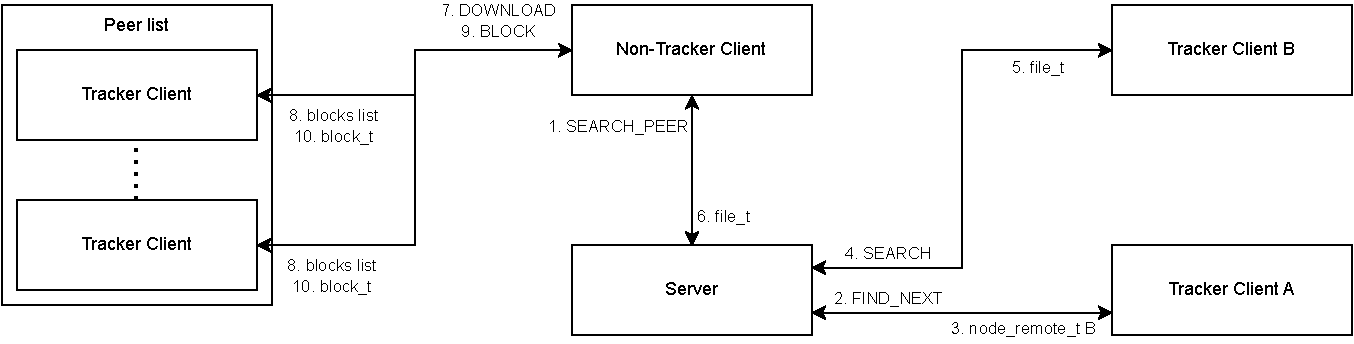
\includegraphics[width=\textwidth]{non_tracker_download.drawio.pdf}
\caption{Download flow for a non-tracker} \label{non_tracker_download}
\end{figure}
\begin{figure}
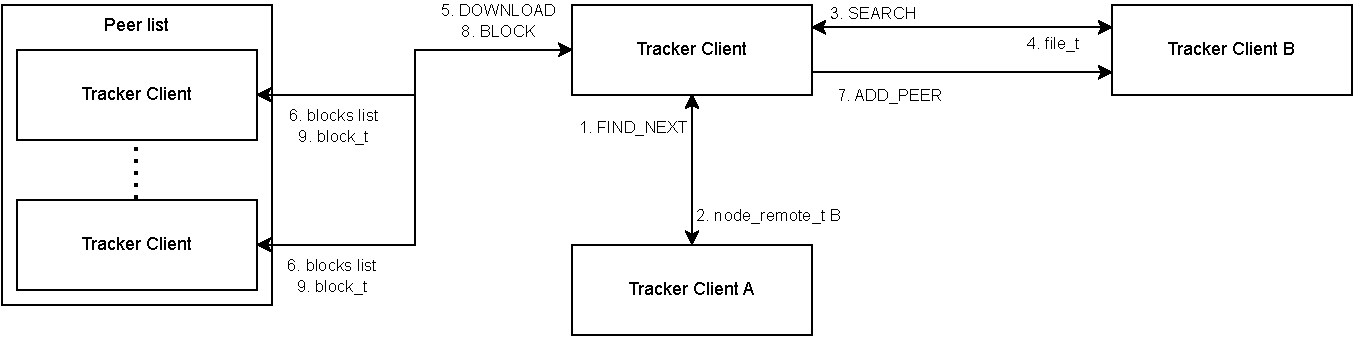
\includegraphics[width=\textwidth]{tracker_download.drawio.pdf}
\caption{Download flow for a tracker} \label{tracker_download}
\end{figure}

The downloader has a pool of threads which actively check for any downloads that are in the \verb|IDLE| state and starts them. After this a download can be either \verb|PAUSED| or \verb|DONE|. \verb|PAUSED| downloads can be retaken by calling the download command again, which will follow the same protocol as above, with the exception that instead of calling \verb|download_init|, only the peers list is reinitialized, because the rest of the data doesn't change.

\subsection{Error system}
Found in \verb|error.h|
There is an error system designed that provides the end user with friendly error messages and provides easy debugging for the developer. Basically, this system is more of a convention than anything else but every function that can return errors must declare a \verb|status| variable which it must modify and return in case of errors or success. In order to check if something returned an error there is the \verb|CHECK| macro which moves the error code in the \verb|status|. Also each error return must print the name of the function and the cause of error, this provides a stack trace. In the main function \verb|ERR| and \verb|ERR_GENERIC| macros are used to print either a specific error message or a generic one in case the error was internal (i.e. the user doesn't care about that error).

\subsection{Logger}
Found in \verb|logger.h|
Logger is a wrapper over \verb|printf| which has three types of logging \verb|LOG|, \verb|LOG_DEBUG|, \verb|LOG_ERROR|. The last 2 can be disabled at compile time through two macros, because these are used only for development purposes.

\subsection{Network abstractions}
Found in \verb|network.h|
In order to speed-up development, there are some abstractions over the simple \verb|read|, \verb|write|, connect sockets and server sockets, which are to be found in this header. 

\subsection{Client module}
Found in \verb|client.h|.
\begin{lstlisting}
typedef struct {
    struct sockaddr_in bootstrap_addr;  // address of the server

    downloader_t downloader;            // downloader module
    tracker_t *tracker;                 // tracker module
} client_t;
\end{lstlisting}
The client module is pretty simple, it stores the address of the server (recall that a new connection is made for each request). The downloader module and tracker module are stored in the client as well. Each client has a list of commands that it can do (some are available only to trackers):
\begin{description}
    \item{\verb|tracker -start|} - starts the tracker module
    \item{\verb|tracker -stop|} - stops the tracker module
    \item{\verb|tracker -stab|} - stabilizes the tracker state as described in \ref{chord_protocol}
    \item{\verb|tracker -state|} - shows the state of the tracker (debug)
    \item{\verb|search [-i FILE_ID] [-n FILE_NAME] [-s FILE_SIZE]|} - send a \verb|SEARCH| request to the server to find a file that matches the \verb|FILE_ID| and contains the \verb|FILE_NAME| and matches the \verb|FILE_SIZE|
    \item{\verb|download -k ID|} - downloads the file with id \verb|ID|
    \item{\verb|download -l|} - list all downloads
    \item{\verb|download -p INDEX|} - pause the download with the specified index from the downloads list
    \item{\verb|upload -p PATH|} - takes the file from \verb|PATH| and uploads it on the network
    \item{\verb|help|} - shows a pretty help message
    \item{\verb|clear|} - clear terminal
    \item{\verb|quit|} - exit application
\end{description}
The download module has been described in detail in \ref{download_protocol}. The \verb|tracker_t| type looks like this:
\begin{lstlisting}
typedef struct {
    // used by threads to know when to stop
    int32_t running;
    pthread_mutex_t running_lock;
    
    pthread_mutex_t lock;               // tracker structure lock

    // local server data
    int32_t fd;
    struct sockaddr_in addr;
    pthread_mutex_t mlock;              // accept lock
    pthread_t tid[THREAD_POOL_SIZE];

    node_local_t node;                  // the dht network local data

    file_list_t files;                  // list of torrent files stored by the tracker
    local_file_list_t local_files;      // list of files that the tracker can transfer upon a download request

    downloader_t *downloader;           // a pointer to the downloader module of the client
} tracker_t;
\end{lstlisting}
Each tracker stores the Chord network state in \verb|node|, a list of torrent files that are handled by the tracker in \verb|files| and the uploads of the tracker in \verb|local_files|. It also has a pointer to the client downloader because, as described in \ref{download_protocol}, the download protocol is a bit different between trackers and non-trackers, so there are two different functions for the two.

\subsection{Server}
\begin{lstlisting}
#define THREAD_POOL_SIZE 2

typedef struct {
    pthread_mutex_t lock;   // struct lock

    int32_t fd;
    struct sockaddr_in addr;

    pthread_mutex_t mlock;
    pthread_t tid[THREAD_POOL_SIZE];

    list_t clients;
    node_t *client_read; // read cursor to "uniformly" distribute peers to new clients

    file_list_t uploads;
} server_t;
\end{lstlisting}
The server uses a pool of threads to handle requests concurrently using accept in each thread. Regarding the state of the server, it stores in memory the list of currently connected trackers in \verb|clients|. If a non-tracker wants to become a tracker, it must ask the server to find a peer in the network and this is the peer that will be used by the client to \verb|join| the network. This peer is stored in \verb|client_read| for fast access and it is basically a pointer that walks circularly the \verb|clients| linked list. Some of the behaviours of the server (such as the network join method and \verb|client_read| cursor) are inspired from BitTorrent \cite{ref_url4,ref_url5,ref_url6}.

The server also stores information about all downloads in order to allow for searches in \verb|uploads|. A search is done by sending a \verb|SEARCH| request with a query and a list of results may be returned, which looks like this:
\begin{lstlisting}
typedef struct {
    // fields to ignore in query
    // if we want to query only by name, then ignore_id = ingore_size = 1
    int32_t ignore_id, ignore_name, ignore_size;
    key2_t id;
    char name[512];
    uint64_t size;
} query_t;

typedef struct {
    key2_t id;
    char name[512];
    uint64_t size;
} query_result_t;
\end{lstlisting}

\section{Conclusions} \label{conclusions}
Currently there are many things that may be improved about the app, such as:
\begin{itemize}
    \item The download algorithm may be improved as currently for each \verb|BLOCK| request, the tracker must find the file referenced by the id and then open that file and read that block. A more efficient solution would be if a separate thread would handle the communication with the handler, as such, the need to search and open the file repeatedly are removed and the transfers can be more fluent.
    \item A better command parser with command descriptions, short and long flags, typed flags and better user input checks.
    \item Download statistics such as download speed, upload/download rate.
    \item Usage of a database system (I am thinking about implementing one myself) as currently the server holds it's data in-memory.
    \item The code allows the user to use torrent files obtained from other sources than the server or the Chord network (i.e. from a website), but there is currently no command that allows loading such files and downloading them.
    \item Implement redundancy for the Chord network keys because if a tracker fails unexpectedly it's data will be lost and so the torrent files that it handled.
\end{itemize}

\pagebreak

\section{Bibliographic References} \label{references}
\begin{thebibliography}{99}
    \bibitem{ref_url1} SHA256 implementation, \url{https://github.com/B-Con/crypto-algorithms/tree/master}, last accessed 14/12/2023
    \bibitem{ref_url2} Peer to peer overview, \url{http://www.rogerclarke.com/EC/P2POview.html}, last accessed 14/12/2023
    \bibitem{ref_url3} Peer to peer overview, \url{https://en.wikipedia.org/wiki/Peer-to-peer}, last accessed 14/12/2023
    \bibitem{ref_url4} BitTorrent, \url{https://en.wikipedia.org/wiki/BitTorrent}, last accessed 14/12/2023
    \bibitem{ref_url5} BitTorrent DHT Bootstrap Server, \url{https://engineering.bittorrent.com/2013/12/19/dht-bootstrap-update/}, last accessed 14/12/2023
    \bibitem{ref_url6} BitTorrent DHT Bootstrap Server source code, \url{https://github.com/bittorrent/bootstrap-dht/blob/master/src/main.cpp}, last accessed 14/12/2023
    \bibitem{ref_url7} Consistent hashing, \url{https://en.wikipedia.org/wiki/Consistent\_hashing}, last accessed 14/12/2023
    \bibitem{ref_url8} DHT, \url{https://en.wikipedia.org/wiki/Distributed\_hash\_table}, last accessed 14/12/2023
    \bibitem{ref_url9} Chord protocol, \url{https://en.wikipedia.org/wiki/Chord\_(peer-to-peer)}, last accessed 14/12/2023
    \bibitem{ref_url10} Chord protocol, \url{https://pdos.csail.mit.edu/papers/chord:sigcomm01/chord\_sigcomm.pdf}, last accessed 14/12/2023
\end{thebibliography}
\end{document}

